\subsection{MetaNetwork}
By clicking toolsets and then MetaNetwork,
users are directed to the MetaNetwork home page, 
as Figure~\ref{fig:MetaNetworkHome}.
MetaNetwork aims to detect gene modules with different co-expression patterns under different biological conditions. 
We use the correlation to quantify the co-expression level. 
High correlation in a gene module, either positive or negative, means the genes inside this module are functionally related, 
which may indicate they are controlled by the same transcriptional regulatory program, or member of the same pathway.
The R package for the MetaNetwork module can be found at \url{https://github.com/metaOmics/MetaNetwork}.

\begin{figure}[H]
\begin{center}
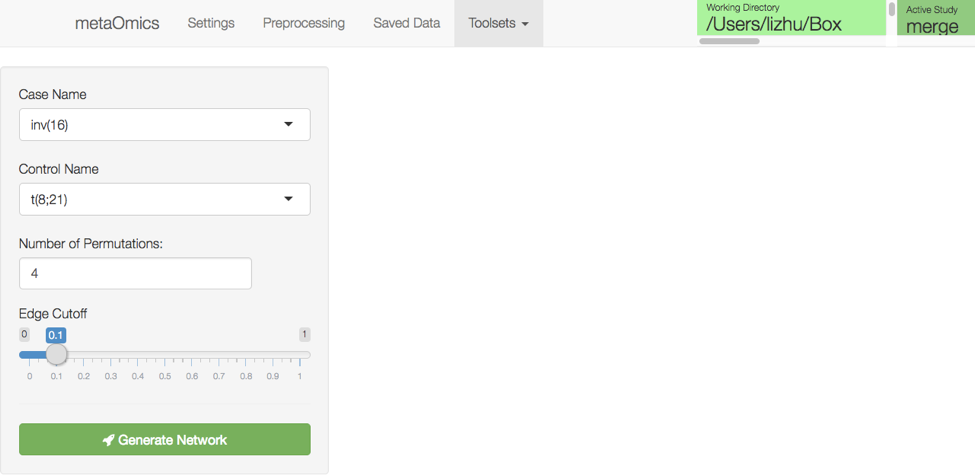
\includegraphics[scale=0.5]{./figure/MetaNetwork/MetaNetworkHome}
\caption{MetaNetwork homepage}
\label{fig:MetaNetworkHome}
\end{center}
\end{figure}

MetaNetwork includes three steps to get differentially co-expressed networks,
including (1) generate network, (2) search for basic modules, and (3) assemble supermodules. 
The left side of Figure~\ref{fig:MetaNetworkHome} is the control panel of \ref{step:MetaDCN1}. 
The control panel for \ref{step:MetaDCN2} and \ref{step:MetaDCN2} will show up after the previous step is completed.
The explanation of the complete list of all options are in Section~\ref{sec:completeList_MetaNetwork}


\subsubsection{Procedure}

\begin{steps}
\item \textbf{Generate Network}
\label{step:MetaDCN1}
The first step of MetaNetwork is to generate the co-expression network. 
In this step, the network for permuted data will also be generated. 
Users need to select case and control names, the number of permutations, and edge cutoff which determines the proportion of edges to be kept in the network. 
Permutations are used to generate the null distribution for edge energy, 
which will be further used to calculate edge FDR. 
Increasing the number of permutations can provide a more accurate FDR estimate but also increases the computation time if a single CPU is used. 
Given a reasonable number of edges, 3-10 permutations are recommended.
A quantile cutoff for edge correlation is applied to decide if an edge exists or not. 
Only edges with correlations above this cutoff will be kept as connected. 
Decreasing the edge cutoff will result in a denser network and add computation time. 
We recommend starting with a large cutoff (looser network), 
especially for large numbers of genes and then gradually decreasing it (increasing network density) for a desirable network.
After clicking the \textbf{Generate Network} button,
the screen will show a message indicating the algorithm is running to generate the network.

\item \textbf{Search for basic modules}
\label{step:MetaDCN2}

The next step is to search for basic modules.
Advanced options (users are recommended not to change) 
include the number of repeats used for each initial seed modules (Number to repeat),
the maximim Monte Carlo steps for the simulated annealing algorithm (MC Steps),
and the maximum pairwise Jaccard index allowed for basic modules (Jaccard Cutoff), as shown in Figure~\ref{fig:MetaNetworkstep2}.
When searching for basic modules, 
we try multiple repeats with different seeds to avoid local optimum. 
Increasing the repeat times will generate more basic modules but will again raise the computation burden. 
We recommend starting with the default number of three repeats, 
and only increasing it if the number of basic modules detected is too small.
If two repeats from the Monte Carlo simulation are very similar (with a Jaccard index greater than the cutoff),
only one repeat with stable configuration (low energy) will be kept in the analysis.
Users are advised to use the default options (Jaccard index cutoff = 0.8).
Explanations of these technical terms are omitted in this tutorial,
but readers can refer to \cite{zhu2016metadcn} for details.
After clicking the \textbf{Search for basic modules} button in Figure~\ref{fig:MetaNetworkstep2}, 
the screen will show a message indicating the algorithm is running to search for basic modules.
This step is computationally demanding, depending the on gene size.
After this step is done,
tables summarizing two kinds of basic modules: one highly connected in cases but loosely connected in control, and the other one with reverse pattern. 

\begin{figure}[H]
\begin{center}
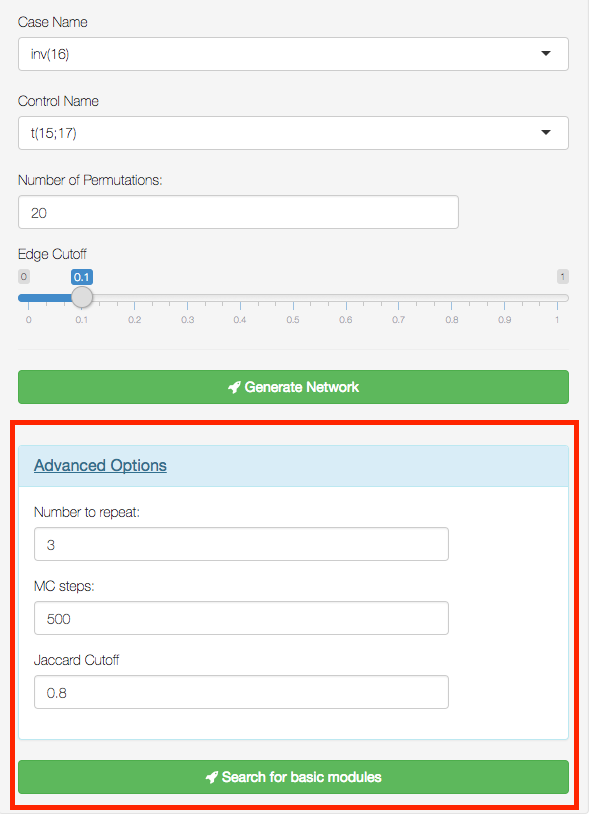
\includegraphics[scale=0.35]{./figure/MetaNetwork/MetaNetworkstep2}
\caption{MetaNetwork control panel for search for basic modules}
\label{fig:MetaNetworkstep2}
\end{center}
\end{figure}

A search for basic modules can be time consuming, 
especially if a large number of genes are used. 
After this step is done, the screen will show a table of basic modules higher correlated in case and a table of basic modules higher correlated in control, as in Figure~\ref{fig:MetaNetworkBM}. 

\begin{figure}[H]
\begin{center}
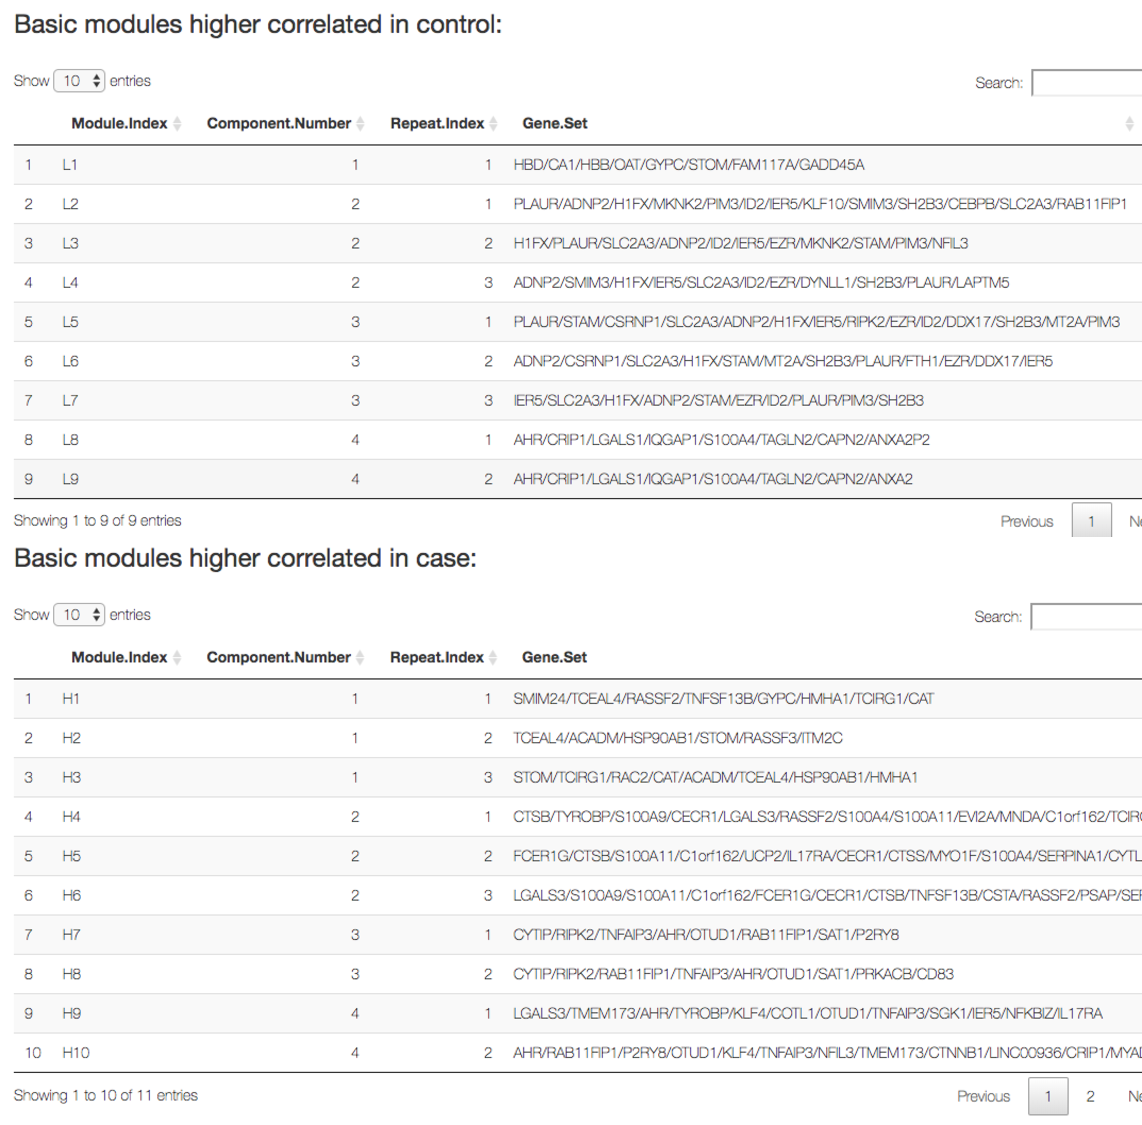
\includegraphics[scale=0.9]{./figure/MetaNetwork/MetaNetworkBM.pdf}
\caption{MetaNetwork output from search for basic modules step.
These modules higher correlated in case are labeled as H1, $\ldots$, H6,
and the modules higher correlated in control are labeled as L1, $\ldots$, L6.
The component number and repeat index are for intermediate indexes.
The actual gene sets are listed for each basic module.
}
\label{fig:MetaNetworkBM}
\end{center}
\end{figure}

\item \textbf{Assemble supermodules}
\label{step:MetaDCN2}

After searching for basic modules step, 
the control panel becomes what is shown in Figure~\ref{fig:MetaNetworkstep3}. 
The last step is to assemble supermodules. 
Users can decide the FDR cutoff to select basic modules for supermodule assembly. 
In Figure~\ref{fig:MetaNetworkstep3}, 
MCStep denotes the maximum number of iterations in the simulated annealing searching algorithm. 
A default 500 is recommended. 
After clicking the \textbf{Assemble supermodules} button, 
the screen will show message indicating the algorithm is running to assemble supermodules.
A table for basic modules, supermodules, and their network visualization will be shown on the right panel of the screen.
MetaNetwork automatically creates files of top supermodules designed to input to a Cytoscape plug-in ``MetaDCNExplorer"
(\url{http://tsenglab.biostat.pitt.edu/software.htm}) for improved visualization and dynamic exploration.

\begin{figure}[H]
\begin{center}
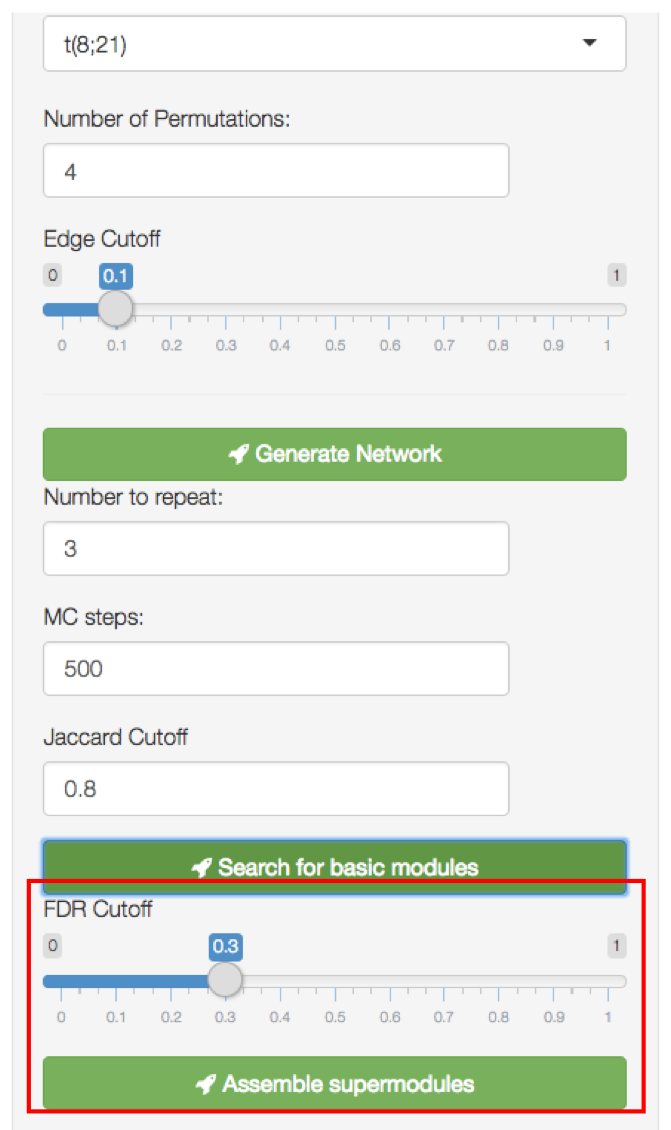
\includegraphics[scale=0.5]{./figure/MetaNetwork/MetaNetworkstep3}
\caption{MetaNetwork control panel for the ``Assemble supermodules" step}
\label{fig:MetaNetworkstep3}
\end{center}
\end{figure}



\end{steps}

\subsubsection{Results}

We used the leukemia data to demonstrate the MetaNetwork module.
After merging the three datasets by filtering out 80\% of genes by mean and 80\% by variance, 206 genes remained.
In this example we only compared two phenotypes: inv(16) and t(15;17).
Detailed descriptions of these studies can be found in Table~\ref{tab:realDataLeukemia}. 
In general, the MetaNetwork tool is time consuming for large datasets (for both the ``network generation" and ``search for basic modules" steps).
We generally suggest users carefully restrict the number of genes 
(e.g., less than a thousand) for a test run before applying them to a large gene set.
By default, all outputs and several interim RData files will be automatically saved to the folder named ``MetaNetwork" under the working directory specified in Section~\ref{sec:setting}.




After the  \textbf{Generate Network} step is done, 
no output will show up on the screen. Instead, a message box will show up indicating several Rdata files are saved in the MetaNetwork folder. 
After the \textbf{Search for basic modules} step is done, the screen will show a table of basic modules higher correlated in case or control, 
as in Figure~\ref{fig:MetaNetworkBM}. 
After the \textbf{Assemble supermodules} assembly is done, 
the screen will show a table of supermodules (Figure~\ref{fig:MetaNetworksuper}). 
Users can also select basic modules to plot (Figure~\ref{fig:MetaNetworkBMplot}). 
Meanwhile several files will be saved in the MetaNetwork folder.
Detailed explanations of all these intermediate files are described in Section~\ref{sec:completeList_MetaNetwork}.

\begin{figure}[H]
\begin{center}
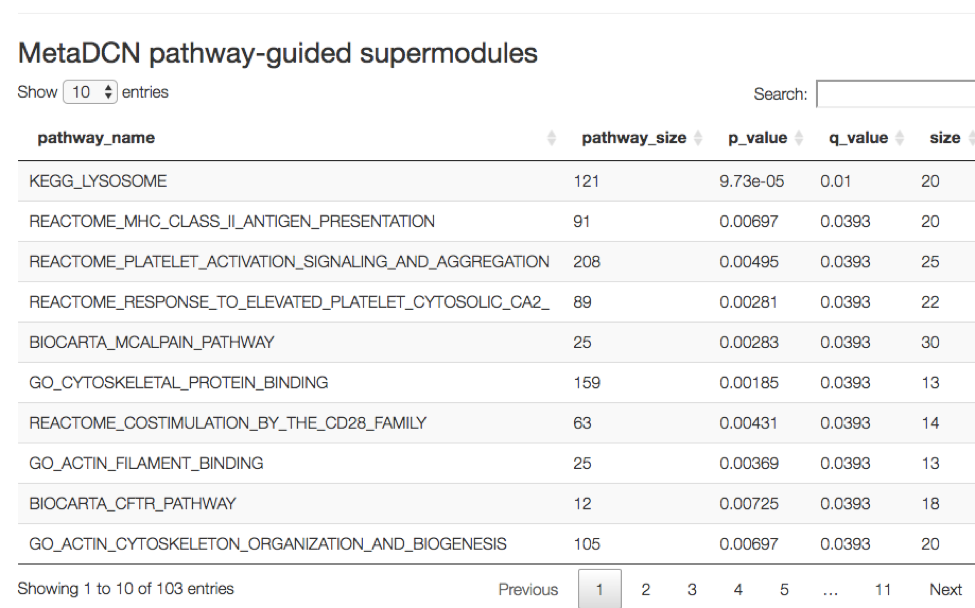
\includegraphics[scale=0.3]{./figure/MetaNetwork/MetaNetworksuper.png}
\caption{MetaNetwork supermodules table.
The second column shows the pathway size.
The third and fourth column show the p-value and q-value of the detected supermodule.
The last column is the size of the supermodule.
}
\label{fig:MetaNetworksuper}
\end{center}
\end{figure}

\begin{figure}[H]
\begin{center}
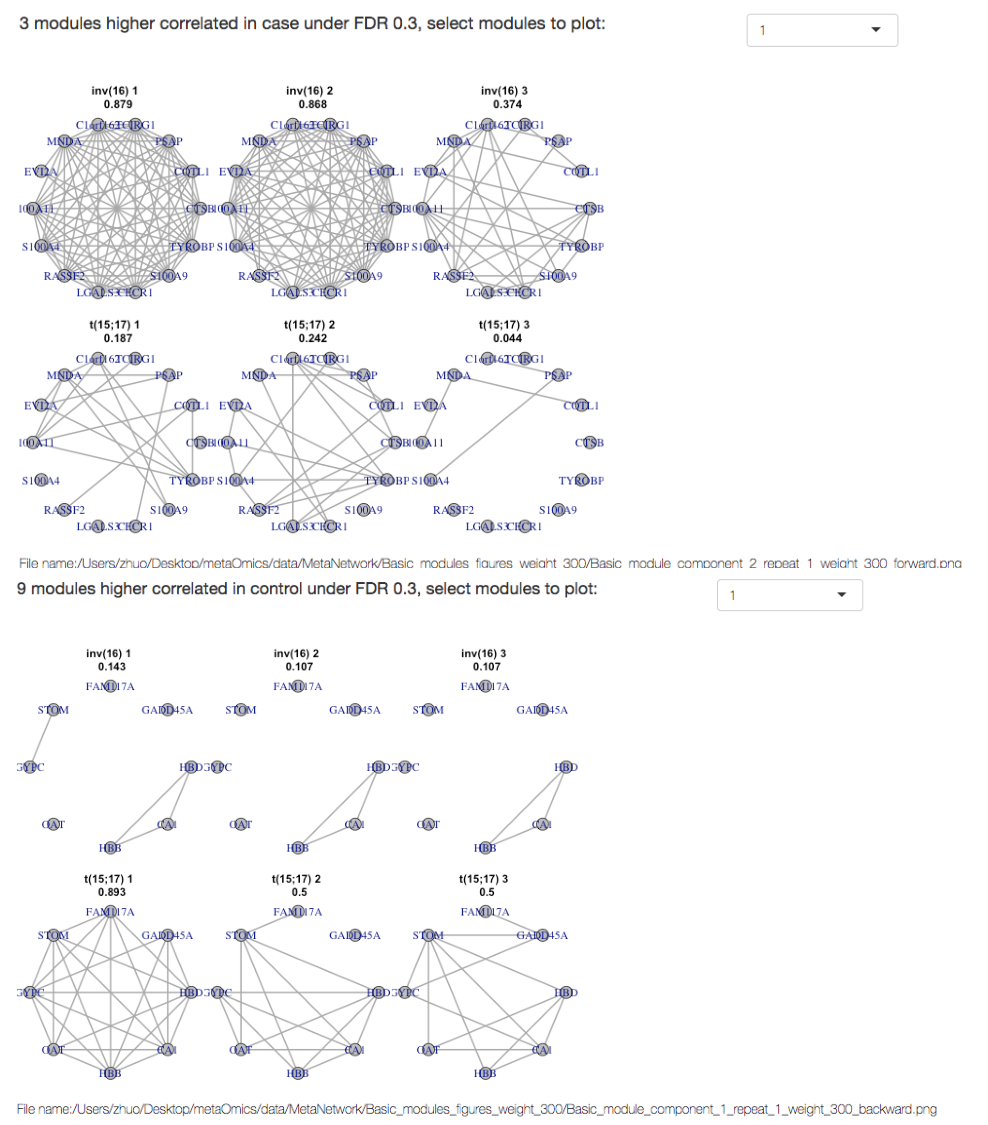
\includegraphics[scale=0.7]{./figure/MetaNetwork/MetaNetworkBMplot.pdf}
\caption{MetaNetwork select basic modules to plot.
Each dot represents a gene.
An edge represents the two genes are highly correlated.
The network density is marked on top of each network.
The top three modules show higher correlation in inv(16), 
and the bottom three modules show higher correlation in t(15:17).
}
\label{fig:MetaNetworkBMplot}
\end{center}
\end{figure}
